\section{Auswertung} 

\subsection{Reflexionsgesetz}

\begin{flushleft}
    Das Reflexionsgesetz wird untersucht. Dabei wird der Lichtstrahl, welcher sich an der Grenzfläche reflektieren sollte untersucht.
    Dazu wurden sieben Einfallswinkel $\alpha_{1}$ an den Reflexionswinkel $\alpha_{2}$, in Tabelle \ref{Tabelle2} aufgenommen.
\end{flushleft}

\begin{table}[H]
    \centering
    \caption{Die Messwerte zur Untersuchung des Reflexionsgesetzes.} 
    \label{Tabelle2}
    \begin{tabular} {c  c}
        \toprule
        {$ \alpha_{1} \mathbin{/} \unit{\degree} $} &
        {$ \alpha_{2} \mathbin{/} \unit{\degree} $} \\
        \midrule
        70 & 69,5 \\
        60 & 60 \\
        50 & 49,5 \\
        40 & 40 \\
        35 & 35 \\
        30 & 30 \\
        20 & 20 \\
        \bottomrule
    \end{tabular} 
\end{table}

\subsection{Brechungsgesetz und Strahlversatz}

\begin{align}
    \intertext{Sobald ein Lichtstrahl von einem optisch dünneren Medium in ein optisch dichteres Medium übergeht, so wird der Lichtstrahl zum Lot hin gebrochen.
    Das Brechnungsgesetz lautet}
    \frac{\sin(\alpha)}{\sin(\beta)} = \text{n}\,, \label{7}
    \intertext{mit $\text{n}_{1} = \text{n}$ und $\text{n}_{2} = \text{n}$, wenn das optisch dünnere Medium Luft ist.
    In der Tabelle \ref{Tabelle3} wurden sieben Einfallswinkel $\alpha$ mit den Brechungswinkel $\beta$ aufgenommen, ebenso den Strahlversatz s des Lichtstrahls.
    Der Strahlversatz, welcher sich durch die Formel}
    \text{s} = \text{d}\,\frac{\sin(\alpha - \beta)}{\cos(\beta)}\,, \label{8}
    \intertext{berechnen lässt erfolgt wenn ein Teil des Lichtstrahls durch die planparallele Platte hin durch geht und an beiden Grenflächen gebrochen wird.
    Dabei wird die Richtung erhalten.
    Der Abstand der Grenzflächen beträgt $\text{d} = 0,0585\,\unit{\meter}$.
    Die Werte der Brechungsindizes n werden nach den Formeln}
    \overline{\text{x}} = \frac{1}{\text{N}} \sum_{\text{i}=1}^{\text{N}} \text{x}_{\text{i}} \label{9} \\
    \increment \overline{\text{x}} = \frac{1}{\sqrt{\text{N}}}\,\,\sqrt{\frac{1}{\text{N}-1}\,\sum_{\text{i}=1}^{\text{N}} \left(\text{x}_{\text{i}} - \overline{\text{x}}\right)^2} \label{10}
    \intertext{gemittelt und die dazugehörige Abweichung bestimmt.} \notag
\end{align}

\begin{table}[H]
    \centering
    \caption{Die Messwerte die Brechungsindizes und die Strahlversetzungen.} 
    \label{Tabelle3}
    \begin{tabular} {c  c  c  c}
        \toprule
        {$ \alpha \mathbin{/} \unit{\degree} $} &
        {$ \beta  \mathbin{/} \unit{\degree} $} &
        {$ \text{n} $} &
        {$ \text{s} $} \\
        \midrule
        70 & 39,0 & 1,49 & 0,038  \\
        60 & 35,5 & 1,49 & 0,029  \\
        50 & 30,5 & 1,50 & 0,022  \\
        40 & 25,5 & 1,49 & 0,016  \\
        35 & 22,5 & 1,49 & 0,013  \\
        30 & 19,5 & 1,49 & 0,011  \\
        20 & 13,5 & 1,46 & 0,006  \\
        \bottomrule
    \end{tabular} 
\end{table}

\begin{align*}
    \intertext{Daraus folgt für den Brechungsindex}
    \text{n} = (1,4871 \pm 0,0116)\,.
    \intertext{Somit beträgt die Geschwindigkeit im Plexiglas nach der Formel (\ref{1})}
    \text{v} = 2,0159 \cdot 10^{8}\,\frac{\unit{\meter}}{\unit{\second}}\,.
\end{align*}

\subsection{Brechung am Prisma}

\begin{align*}
    \intertext{Ein Prisma wird durch nicht parallele Flächen begrenzt.
    Beim Durchgang durch das Prisma erfährt der Strahl die Ablenkung $\delta$, mit}
    \delta = (\alpha_{1}+ \alpha_{2}) - (\beta_{1} + \beta_{2})\,.
    \intertext{Der Einfallswinkel $\alpha_{1}$ und der Austrittswinkel $\alpha_{2}$ werden gemessen.
    Die Winkel $\beta_{1}$ und $\beta_{2}$ werden über da Brechungsgesetz $\sin(\alpha) = \text{n} \cdot \sin(\beta)$ und die Winkelbeziehung $\beta_{1} + \beta_{2} = \gamma$ hergeleitet.
    Gewählt wird ein Winkelbereich von $10\unit{\degree} \leq \alpha_{1} \leq 60\unit{\degree}$ und das Prisma hat ein brechenden Winkel von $\gamma = 60\unit{\degree}$. 
    Der Brechungsindex beträgt $\text{n}_{\text{theo, Kronglas}} = 1,52$.}
\end{align*}

\begin{figure}[H]
    \centering
    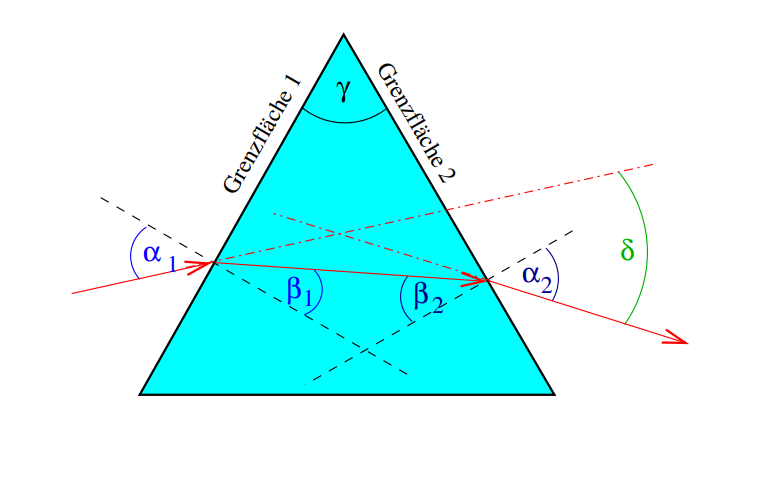
\includegraphics[height=55mm]{bilder/A6.png}
    \caption{Brechung am Prisma \cite{a1}. \label{Abbildung6} }
\end{figure}

\begin{table}[H]
    \centering
    \caption{Messdaten und Berechnungen am Prisma.} 
    \label{Tabelle4}
    \begin{tabular} {c  c  c  c  c  c  c  c}
        \toprule
        {$ \alpha_{1,\text{rot}} \mathbin{/}\unit{\degree}$} &
        {$ \alpha_{2,\text{rot}} \mathbin{/}\unit{\degree} $} &
        {$ \alpha_{1,\text{grün}} \mathbin{/}\unit{\degree} $} &
        {$ \alpha_{2,\text{grün}} \mathbin{/}\unit{\degree} $} &
        {$ \beta_{1,\text{grün},\text{rot}} \mathbin{/}\unit{\degree} $} &
        {$ \beta_{1,\text{grün},\text{rot}} \mathbin{/}\unit{\degree} $} &
        {$ \delta_{\text{grün}} \mathbin{/}\unit{\degree} $} &
        {$ \delta_{\text{rot}} \mathbin{/}\unit{\degree} $}\\
        \midrule
        30 & 79,5 & 30 & 81,0 & 19,20 & 40,80 & 51,0 & 49,5 \\
        35 & 68,2 & 35 & 69,0 & 22,16 & 37,84 & 44,0 & 43,2 \\
        40 & 60,1 & 40 & 60,8 & 25,01 & 34,99 & 40,8 & 40,1 \\
        45 & 53,7 & 45 & 54,3 & 27,72 & 32,28 & 39,3 & 38,7 \\
        50 & 48,2 & 50 & 48,8 & 30,26 & 29,74 & 38,8 & 38,2 \\
        60 & 39,4 & 60 & 39,8 & 34,73 & 25,27 & 39,8 & 39,4 \\
        \bottomrule
    \end{tabular} 
\end{table}

\subsection{Beugung am Gitter}

\begin{align}
    \intertext{Das Laserlicht trifft die Winkelskala des Transmissionsschirmes bei $0\unit{\degree}$.
    Die Ablenkwinkel $\varphi$ können an der Winkelskala direkt abgelesen werden, da der Transmissionsschirm im Kreis um die Skala angeordnet wurde.
    Gemessen werden die Ablenkwinkel und jede Beugungsordnung k für drei Gitterkonstanten.
    Daraus leitet sich für die Wellenlänge}
    \lambda = \text{d}\,\,\frac{\sin(\varphi)}{\text{k}}\,. \label{11}
\end{align}

\begin{table}[H]
    \centering
    \caption{Wellenlängen aus den Ablenkwinkel und Beugungsmaxima.} 
    \label{Tabelle}
    \begin{tabular} {c  c  c  c}
        \toprule
        {}&
        {$ \text{d} = \frac{1}{600}\,\unit{\micro\meter} $} &
        {$ \text{d} = \frac{1}{300}\,\unit{\micro\meter} $} &
        {$ \text{d} = \frac{1}{100}\,\unit{\micro\meter} $} \\
        \hline
        {}&
        {$ \varphi \mathbin{/} \unit{\degree}$} &
        {$ \varphi \mathbin{/} \unit{\degree}$}  &
        {$ \varphi \mathbin{/} \unit{\degree}$}  \\
        \midrule
        roter Laser & 23,2 & 34   & 14,6  \\
                    & 0,40 & 22   & 7,1   \\
                    &      & 10,8 & 3,6     \\
                    &      & 0,20 & 0       \\
                    & $\to \lambda = 656\,\unit{\nano\meter}$ & $\to \lambda = 621\,\unit{\nano\meter}$ & $\to \lambda = 630\,\unit{\nano\meter}$  \\
                    \hline
        grüner Laser & 19,5 & 27,9 & 12  \\
                     & 0,3  & 23,2 &  8,9 \\
                     &  & 9    & 6,8 \\
                     &  & 0,1  & 2,9 \\
                     &  &      & 0,1 \\
         & $\to \lambda = 556\,\unit{\nano\meter}$ & $\to \lambda = 519\,\unit{\nano\meter}$ & $\to \lambda = 519\,\unit{\nano\meter}$ \\
        \bottomrule
    \end{tabular} 
\end{table}
